\documentclass{beamer}
\usetheme{default}
\usepackage[ngerman]{babel}
\usepackage[utf8x]{inputenc}
\usepackage{pgf}

\title{Softwareprojekt 2 Abschlusspräsentation}
\subtitle{Gruppe WOYM}
\date{08.02.2015}
\author{Tim Hansen\\ Adrian Lück\\ Jurij Schmidt}
\institute{Universität Bremen}
\titlegraphic{
\includegraphics[width=2cm,height=2cm]{../WOYM.png}}
\setbeamertemplate{footline}[text line]{%
  \parbox{\linewidth}{\vspace*{-8pt}\hfill\insertshortauthor\hfill\insertpagenumber}}
\setbeamertemplate{navigation symbols}{}
\begin{document}
\maketitle

\section{Projektverlauf}
\begin{frame}
\frametitle{Gliederung}
\tableofcontents[currentsection]
\end{frame}



\section{Statistiken}

\begin{frame}
\frametitle{Gliederung}
\tableofcontents[currentsection]
\end{frame}

\begin{frame}
\frametitle{Commits nach Jahr}
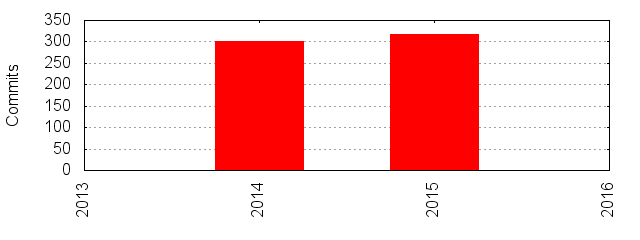
\includegraphics[width=\textwidth]{images/commits_by_year.png}
\end{frame}

\begin{frame}
\frametitle{Commits nach Wochentagen}
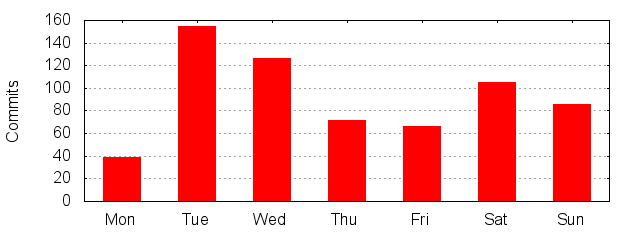
\includegraphics[width=\textwidth]{images/day_of_week.png}
\end{frame}

\begin{frame}
\frametitle{Commits nach Uhrzeit}
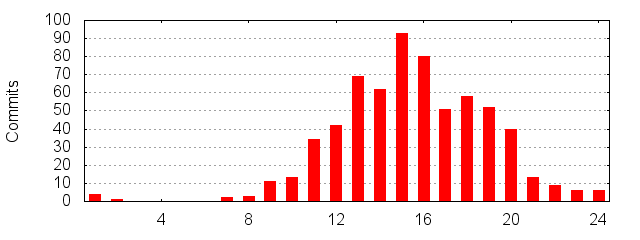
\includegraphics[width=\textwidth]{images/hour_of_day.png}
\end{frame}

\begin{frame}
\frametitle{Aktivität nach Wochen}
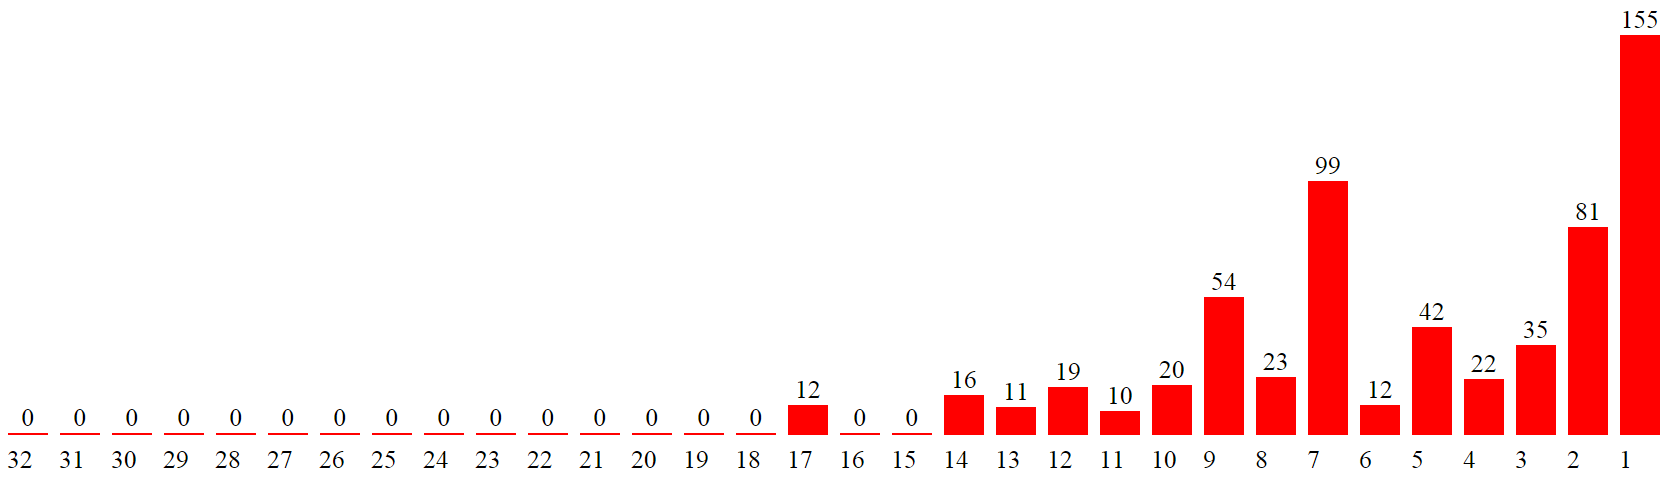
\includegraphics[width=\textwidth]{images/weekly_activity.png}
\end{frame}

\begin{frame} 
  \frametitle{Lines of Code}
  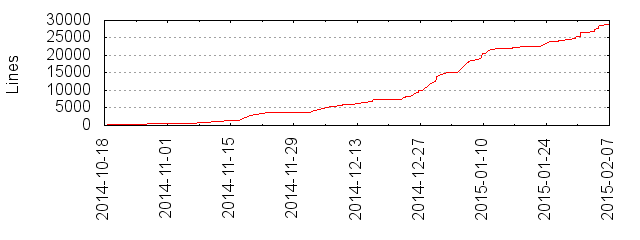
\includegraphics[width=\textwidth]{images/lines_of_code.png}
\end{frame}

\begin{frame}
\frametitle{Lines of Code nach Dateitypen}
\renewcommand{\arraystretch}{2}
\begin{table}
\centering
\begin{tabular}{ccc}
Java: & 24.357 & 84,68 \%\\
XHTML: & 3.670  & 12,76 \%\\
Sonstige: & 718  & 2,56 \%\\
\hline\hline
Insgesamt: & 28.745 & 100 \%\\
\end{tabular}
\end{table}
\end{frame}

\section{Fazit}
\begin{frame}
\frametitle{Gliederung}
\tableofcontents[currentsection]
\end{frame}

\end{document}